\section{Fundamental tools for folding} \label{sec:folding}
In this section, we explore the different ways one can fold a given crease pattern, and derive objectives to control them.


\subsection{Curved folding from the view of the crease} \label{sec:curved_folding_from_a_curve}
Let $\Gamma(t)$ be a curve on a smooth developable surface $S$,  let $\gamma(t)$ be its flattened curve, $k(t)$ its curvature, and $k_g(t)$ its geodesic curvature such that $k_g(t) = k(t) \cos(\alpha(t))$ for some $\alpha \neq 0$. This implies that at each point along $\Gamma(t)$, the tangent planes of $S$ make an angle of $\alpha$ with the osculating planes of $\Gamma(t)$. One can switch this point of view: start with a flat curve $\gamma(t)$, isometrically embed the curve in $\mathbb{R}^3$ and construct a developable surface by reconstructing the planes at each point. As long as the crease is curved, i.e. has some normal curvature such that $k(t) > k_g(t)$ and $\alpha(t) \neq 0$ then there are 2 distinct planes containing $\Gamma'(t)$ and forming an angle of $\alpha(t)$ with the curve's osculating plane. Therefore, one can locally construct two different smooth developable surfaces passing through $\Gamma(t)$ with $\gamma(t)$ as its flattening. Alternatively, one can construct a folded surface by a consistent smooth choice of a different tangent plane for each "side" of the curve (see Fig. \ref{fig:curved_fold_through_curve}) \cite{more_on_paper}. The tangent planes from both sides are reflections of one another through the osculating plane of the curve \cite{curved_folding_kilian}.

\begin{figure} [h]
	\centering
	\includegraphics[width=0.7\linewidth]{figures/curved_fold_through_curve.pdf}
	\caption{(TODO BETTER FIG) Left: A flattened curve in 2D. Right: A small neighbourhood around an embedding of the curve in $\mathbb{R}^3$, its osculating plane and two options to extend a the curve to developable surface by constructing the 2 planes containing the curve's tangent and making an angle of $\alpha(t)$  with the osculating plane. Choosing 2 different tangents along each 'side' of the curve creates discontinuities along the curve and a curved folded surface.}
	\label{fig:curved_fold_through_curve}
\end{figure}

%Two intersecting developable surfaces can be flattened along their intersection if the intersected curve have the same geodesic curvature on both surfaces. 
\subsection{The smooth and combinatorial parameters of a single crease}
A single straight crease is rather boring, mathematically speaking. Straight lines can only be folded as in classical origami, i.e. by keeping them straight \cite{demaine_lens}. Hence the folding process of a single fold can be described by a single real number, representing the fold dihedral angle. As detailed in section \secref{sec:curved_folding_from_a_curve}, there are far more degrees of freedom for folding a curved crease; Up to rigid motion, this folding could be described by two smooth \textit{functions}: the curves' curvature $k(t) \geq k_g(t)$ and its torsion $\tau(t)$. Unlike the case of classical origami, the folding angle of a curved crease can vary along the curve. The folded shape is locally not determined only by these two smooth functions as there is an additional \textit{combinatorial} degree of freedom: the choice of a surface at each side (see \figref{fig:curved_fold_through_curve}). There are four options, two of which creates creates discontinuity along the crease. We call one folded configuration a mountain fold and the other a valley fold. %We follow \cite{demaine_lens} to distinguish between the two type of folded configurations by calling one choice a \textit{Mountain} fold and the other a \textit{Valley} fold. %We note that by \cite{demaine_lens}, a fold always consistently stays mountain/valley throughout the entire creased curve. Assuming a given normal orientation, a fold is said to be a mountain fold if the normal of the surface TODO:ADD EXPLANATION. 


%The curvature and torsion also dictates the ruling patterns of the developable surfaces, generally changing while folding and bending the surface. Deforming a curved crease locally determines the shape of both surfaces around it, and the exact regions of surfaces influenced by that fold depend on the ruling patterns themselves. As mentioned, the rulings patterns themselves can change which can smoothly change during the deformation itself. 

%(there's the cone singularity case where a curved fold is more local (as focused on the cone point) but I think this requires the curve to be C^1.. should mention it?

\subsection{The combinatorial parameters of multiple creases}
Curved folding is well understood locally, around a small part of a single curve, as the tangent planes along the curves are reflections of one another through the folded curve osculating plane. Understanding crease patterns globally still remains a challenge. In essence, deforming one patch propagates a global deformation of the patch on the other side of the crease, a process that depends on the ruling patterns. The ruling patterns are formed as the intersections of the tangent planes, and as mentioned the ruling patterns can smoothly change during the deformation itself. When there are multiple creases this process further propagate and dictates the shape of other patches (see \figref{fig:multiple_crease_pattern}). The process becomes more complicated when some creases intersect due to compatibility constraints (see \figref{fig:multiple_crease_pattern}, right figure). Generally speaking, choosing the first mountain/valley assignment of one fold dictates the mountain/valley assignments of the other folds as the location of another creased is fixed (TODO: see if I can cite demaine-tachi or if that is still unpublished). The combinatorial degrees of freedom that then remain are to determine which folds are active, i.e. folded (TODO: see figurebias-stuff).

% Can change the sentence above to not talk about mountain or valley yet, if needed.
% The pictures which will show are then discrete, though the smooth picture is the same. Maybe put the discrete picture in the setup as well.
% A fold is active if nearby tangents are reflections of one another, and is not active if they are the same as there is no discontinuity. (have a figure that is discrete, but explain it is also the same drawing for the smooth case).
% Write down the formula. Write down a flow. State it is inequality hence folding should be done at time = 0 when it is flat, but nevertheless a binary decision. We characterize it by the sign. 
% One can then view a folding-bending process as a smooth flow, i.e. a smooth deformation on a piecewise C^2 developable surface. The choice to make each fold active is only done during time t = 0, whereas otherwise discontinuties arise, and locally remains a curved fold as the equality.
% Problem in using it for a DOG is that we cannot hope to get it exactly. Then present binary representation. Say how it's really good (also goes to zero very fast).
% The binary characterization in the smooth case, motivate more degrees of freedom, and add the algorithm. Then add control for dihedral angles and mountain valley fold.

\begin{figure} [h]
	\centering
	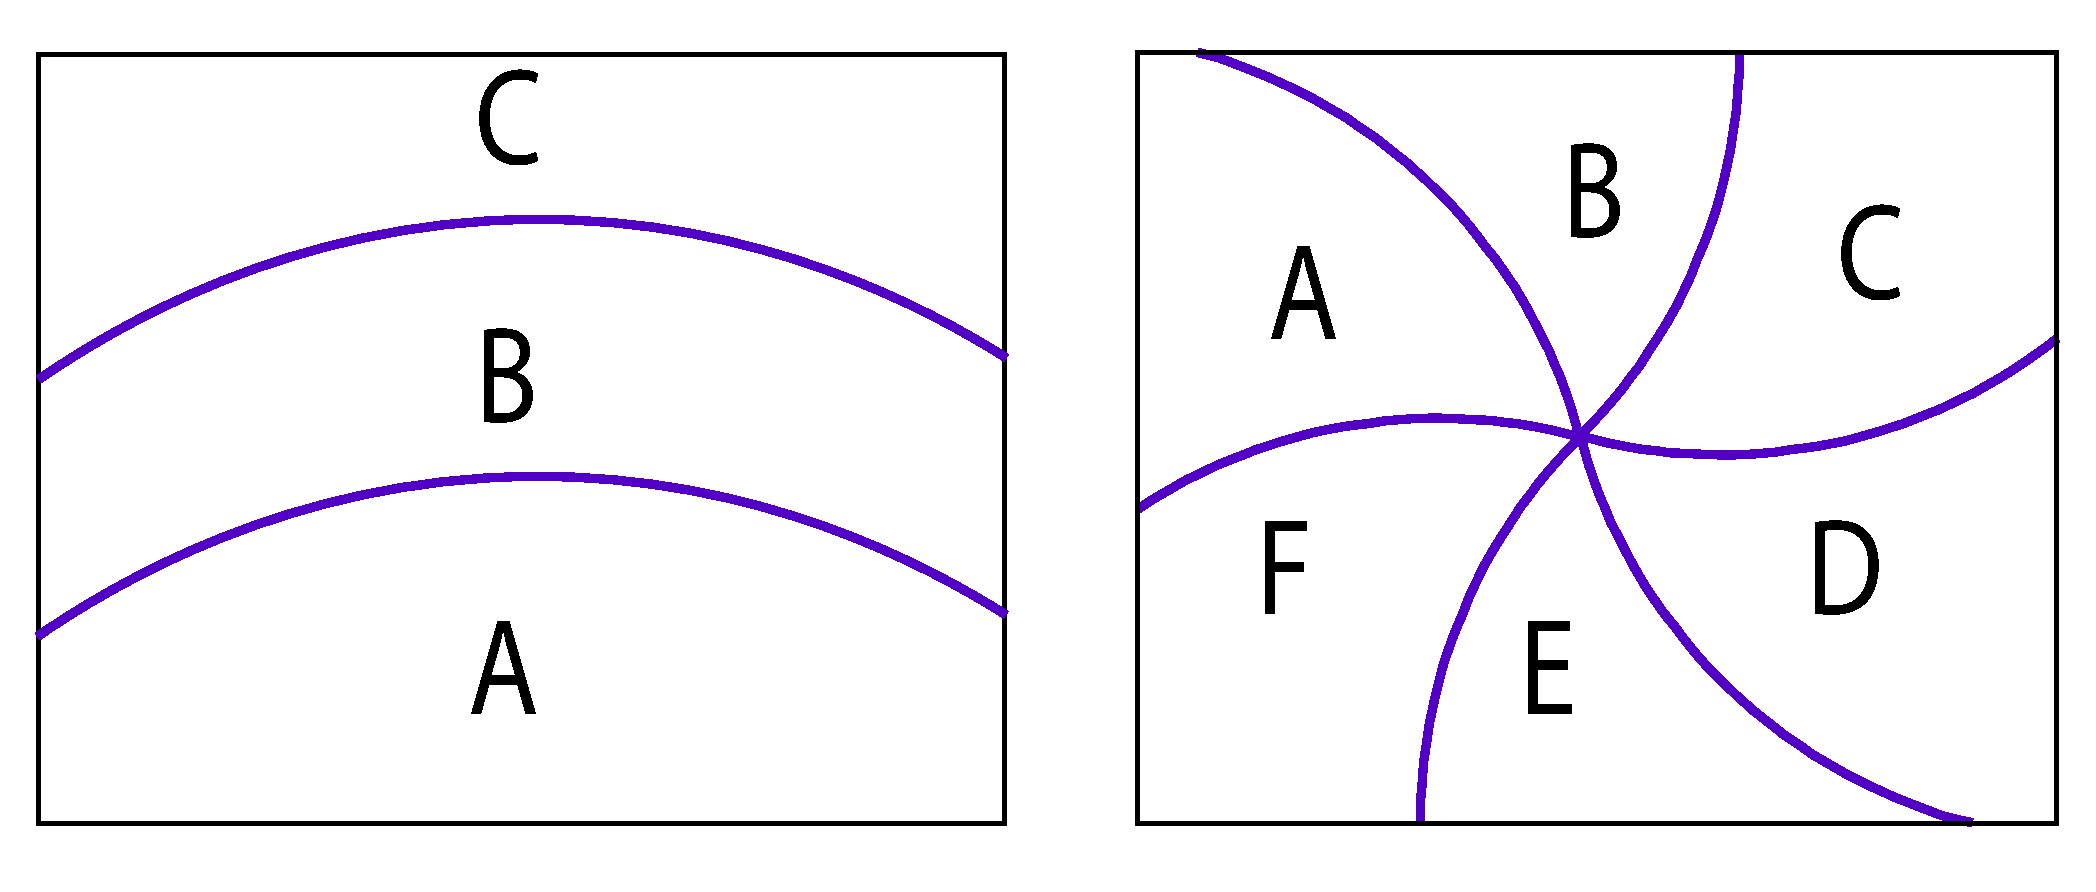
\includegraphics[width=0.7\linewidth]{figures/multiple_crease_patterns}
	\caption{Curved and straight crease patterns, decomposing a pattern into multiple components and intersecting at vertices.}
	\label{fig:multiple_crease_pattern}
\end{figure}
